% \documentclass{book}

\documentclass[12pt]{article}
\usepackage[pdfborder={0 0 0.5 [3 2]}]{hyperref}%
\usepackage[left=1in,right=1in,top=1in,bottom=1in]{geometry}%
\usepackage[shortalphabetic]{amsrefs}%
\usepackage{amsmath}
\usepackage{enumerate}
\usepackage{enumitem}
\usepackage{amssymb}                
\usepackage{amsmath}                
\usepackage{amsfonts}
\usepackage{amsthm}
\usepackage{bbm}
\usepackage[table,xcdraw]{xcolor}
\usepackage{tikz}
\usepackage{float}
\usepackage{booktabs}
\usepackage{svg}
\usepackage{mathtools}
\usepackage{cool}
\usepackage{url}
\usepackage{graphicx,epsfig}
\usepackage{makecell}
\usepackage{array}

\def\noi{\noindent}
\def\T{{\mathbb T}}
\def\R{{\mathbb R}}
\def\N{{\mathbb N}}
\def\C{{\mathbb C}}
\def\Z{{\mathbb Z}}
\def\P{{\mathbb P}}
\def\E{{\mathbb E}}
\def\Q{\mathbb{Q}}
\def\ind{{\mathbb I}}

\graphicspath{ {images9/} }

\begin{document}

\section*{10 March 2017}
Last week's results look good; it seems like we have a method for finding eigenvalues, and they appear to be where we expect/want them to be. Now we repeat our experiment with different paramaters to see what happens, and we also try this on another system.

\subsection*{5th order KdV equation}
We use the 5th order KdV equation with speed $c = 40.9355$. As always, we start with a single pulse for a value of $c$ for which the exact solution is known, and use parameter continuation to increase $c$ to our desired value. Here we use domain size $L = 25$, i.e. interval $[-25, 25]$. For periodic BCs, continuation code was run with $N = 500$ grid points. For Fourier spectral methods, continuation code was run with $N = 128$ grid points.

\subsubsection*{Double Pulse 1}
Double Pulse 1 has two real eigenvalues which are negatives of each other. First we use finite difference methods with periodic BCs. Here is a table of the positive real eigenvalue for increasing values of $N$, the number of grid points. Although we ran the continuation code for 500 grid points, we need $N = 1000$ grid points before we see the appropriate eigenvalue picture. Here is the table of eigenvalues, found using \texttt{eigs}:
\begin{figure}[H]
\begin{tabular}{l|ll}
$N$    & Positive real eigenvalue      &  Difference      \\ \hline
  1000 &       2.8573  &             \\ 
  2000 &       3.3513  &      0.4940 \\ 
  4000 &       3.4627  &      0.1115 \\ 
  8000 &       3.4900  &      0.0272 \\ 
\end{tabular}
\end{figure}

Plotting the log of the difference versus the log of the grid size:
\begin{figure}[H]
\includegraphics[width=8.5cm]{1double1fdeigdiff}
\end{figure}

We have 2nd order convergence, as expected, so that is good. It looks like we are converging to something around 3.5. Now let's try Fourier. Since our matrices will not get too big, we can use \texttt{eig}.

\begin{figure}[H]
\begin{tabular}{l|ll}
$N$    & Positive real eigenvalue      &  Difference      \\ \hline
  128  &        3.5072  &             \\ 
  256  &        3.4990  &      0.0082      \\ 
  512  &        3.4990  &      5.4199e-07  \\ 
  1024 &        3.4990  &      1.0284e-07  \\
  2048 &        3.4990  &      8.9820e-07  \\ 
\end{tabular}
\end{figure}
To test for exponential convergence, we can plot the difference versus the log of the grid size (not shown), but if we do this we don't get a nice straight line. Sine the last three differences are the same order of magnitude, my guess is that we reach max precision quickly with Fourier methods. Fewer than 128 grid points does not produce accurate results. \\

Based on this, it looks like we can use Fourier methods with $N = 512$ as a ``true'' eigenvalue in this case. Let's try a ``true'' value of 3.4990 for the finite difference methods and see what happens. For this we use grid sizes from 1000 to 8000 in increments of 1000.

\begin{figure}[H]
\includegraphics[width=8.5cm]{1double1fdeigtrue}
\end{figure}

Again, we have 2nd order convergence, so Fourier spectral methods give us a nice estimate of the the ``true'' value within about $1e-7$ or so (looking at the differences in the Fourier table). It appears we can do this using only 512 grid points, which is really nice!\\

For reference, here are the eigenfunctions for the pair of real eigenvalues for Double Pulse 1. These use Fourier spectral methods with $N = 1024$. As expected the two eigenfunctions are reflections of each other over the y-axis.
\begin{figure}[H]
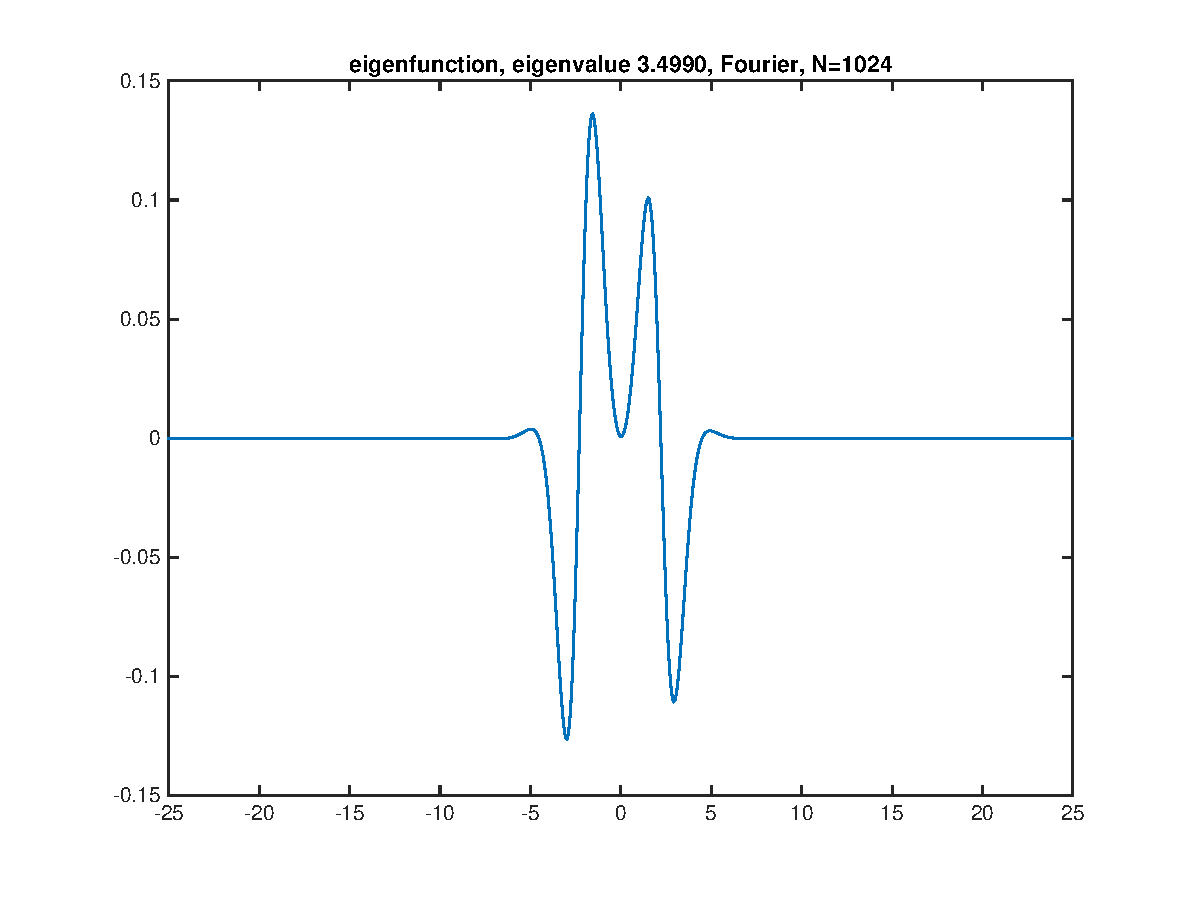
\includegraphics[width=8.5cm]{1double1fouriereigenfnplus}
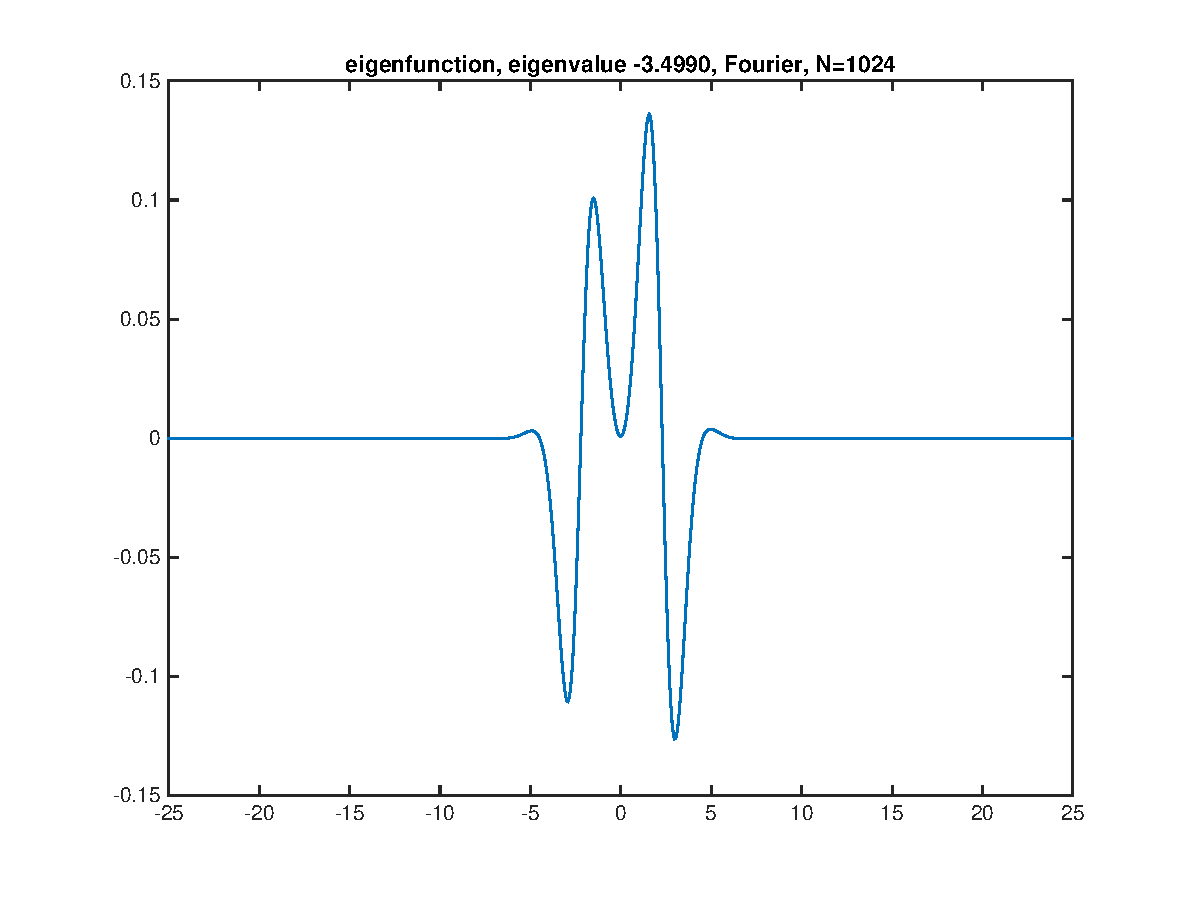
\includegraphics[width=8.5cm]{1double1fouriereigenfnminus}
\end{figure}
Note that these are not symmetric about the y-axis. The eigenfunctions look the same no matter which method or grid size we use.\\

We can also look at the integral of the eigenfunction. We expect it to be 0. Using Fourier spectral methods and the trapezoid rule for numerical integration:

\begin{figure}[H]
\begin{tabular}{lll}
$N$    & Positive real eigenvalue      &  Integral     \\ \hline
  128  &        3.5072  &  -1.3941e-05 \\ 
  256  &        3.4990  &  4.9595e-06  \\ 
  512  &        3.4990  &  -1.7755e-06 \\ 
  1024 &        3.4990  &  6.2412e-07  \\
  2048 &        3.4990  &  -2.7434e-07 \\ 
\end{tabular}
\end{figure}
A plot of the log of the absolute value of the integral versus the log of the mesh size gives a nice straight line, suggesting convergence to 0; however, I have no idea what the order of convergence (about 1.5) means in this case since we have to consider convergence of the Fourier spectral method as well as convergence of the numerical integration scheme.
\begin{figure}[H]
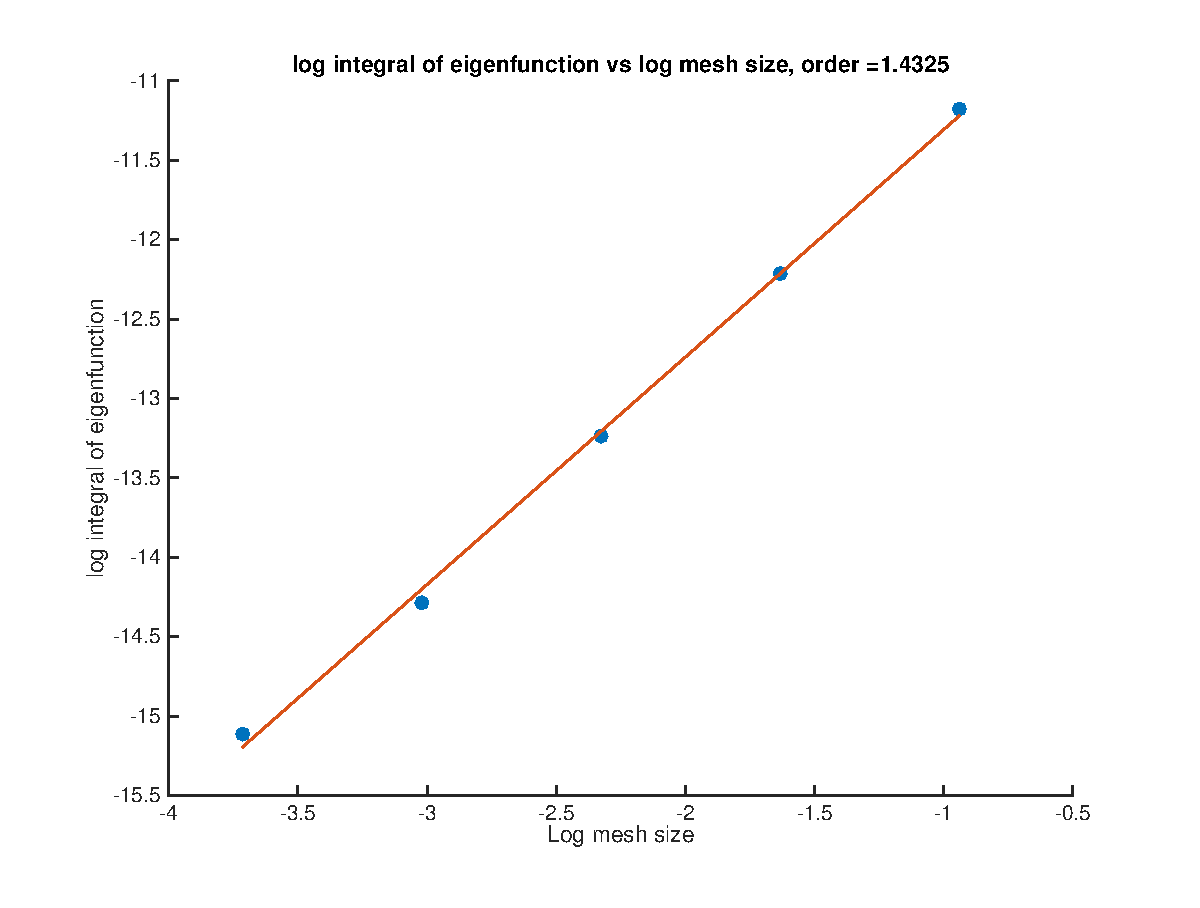
\includegraphics[width=8.5cm]{1double1fouriereigenfnintegralN}
\end{figure}

We can also look at the effect of the domain size $L$ on the integral. Here we keep the mesh size constant, so we double the number of grid points when we double the domain size.

\begin{figure}[H]
\begin{tabular}{llll}
$N$    & $L$    & Positive real eigenvalue      &  Integral     \\ \hline
  256  &  25    &   3.4990  &  4.9595e-06  \\ 
  512  &  50    &   3.4990  &  -5.7404e-07 \\ 
  1024 &  100   &   3.4990  &  -7.9850e-09 \\
  2048 &  200   &   3.4990  &  -7.3953e-12 \\ 
\end{tabular}
\end{figure}

These integrals also appear to be converging to 0, which is nice, although we cannot get a nice linear fit on either a log-log or a semilog plot. \\

Finally, we can look at the effect of the domain size $L$ on the integral with the number of grid points $N$ fixed. For this, we use $N = 2048$.

\begin{figure}[H]
\begin{tabular}{llll}
$N$    & $L$    & Positive real eigenvalue  &  Integral     \\ \hline
       &        &           &  1.0e6 *     \\
  2048 &  25    &   3.4990  &      0.1678 \\ 
  2048 &  50    &   3.4990  &     -0.0700 \\ 
  2048 &  75    &   3.4990  &      0.0156 \\
  2048 &  100   &   3.4990  &      0.0025 \\
  2048 &  125   &   3.4990  &     -0.0005 \\ 
  2048 &  150   &   3.4990  &     -0.0001 \\
\end{tabular}
\end{figure}

On a semi-log plot, we get a nice best-fit straight line, suggesting exponential convergence to 0.
\begin{figure}[H]
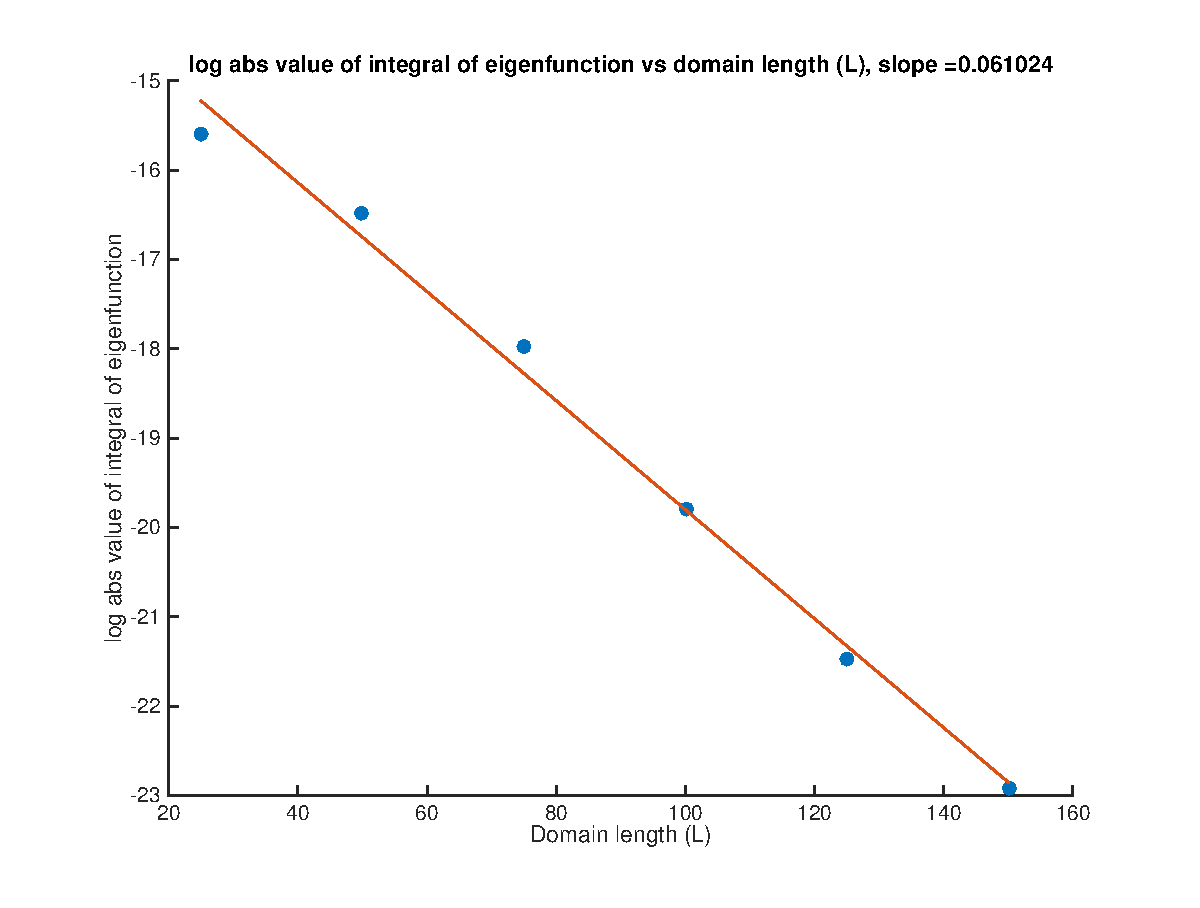
\includegraphics[width=8.5cm]{1double1fouriereigenfnintegralL2048}
\end{figure}


\subsubsection*{Double Pulse 2}
Here we do the same thing we did last time. We use an exponentially weighted space with weight $a = 0.2$ to separate the eigenvalues from the absolute spectrum. First, we use finite difference methods with periodic BCs. The eigenvalue pattern looks exactly the same as it did with $L = 100$, i.e. we have a Left Eigenvalue which appears to be converging to a nonzero value on the imaginary axis, and a Right Eigenvalue which appears to be converging to 0. The eigenfunction of the Right Eigenvalue appears to be an exponentially weighted version of the derivative of the double pulse, so that is good. Here are the eigenvalues. We use grid points from 1000 to 10000 in increments of 1000. Above 10000 or so grid points, it's hard to get good results from \texttt{fsolve}.

\begin{figure}[H]
\begin{tabular}{l|ll}
$N$    & Left eigenvalue      &  Right eigenvalue    \\ \hline
  1000 &   -0.0258 + 2.0161i  &    0.0177 + 1.8828i  \\ 
  2000 &   -0.0081 + 1.1472i  &    0.0062 + 0.9465i  \\ 
  3000 &   -0.0037 + 0.9019i  &    0.0028 + 0.6316i  \\ 
  4000 &   -0.0021 + 0.7987i  &    0.0016 + 0.4739i  \\
  5000 &   -0.0013 + 0.7461i  &    0.0010 + 0.3791i  \\ 
  6000 &   -0.0009 + 0.7160i  &    0.0007 + 0.3159i  \\ 
  7000 &   -0.0007 + 0.6973i  &    0.0005 + 0.2709i  \\ 
  8000 &   -0.0005 + 0.6848i  &    0.0004 + 0.2371i  \\ 
  9000 &   -0.0004 + 0.6762i  &    0.0003 + 0.2109i  \\
 10000 &   -0.0003 + 0.6701i  &    0.0003 + 0.1906i  \\ 
\end{tabular}
\end{figure}
First let's look at the Right Eigenvalue, which we expect to converge to 0 as the mesh size goes to 0 (number of grid points go in infinity). Plotting the log of the absolute value of the Right Eigenvalue vs the log of the mesh size, we see that this is indeed the case. We get first order convergence like we did before.

\begin{figure}[H]
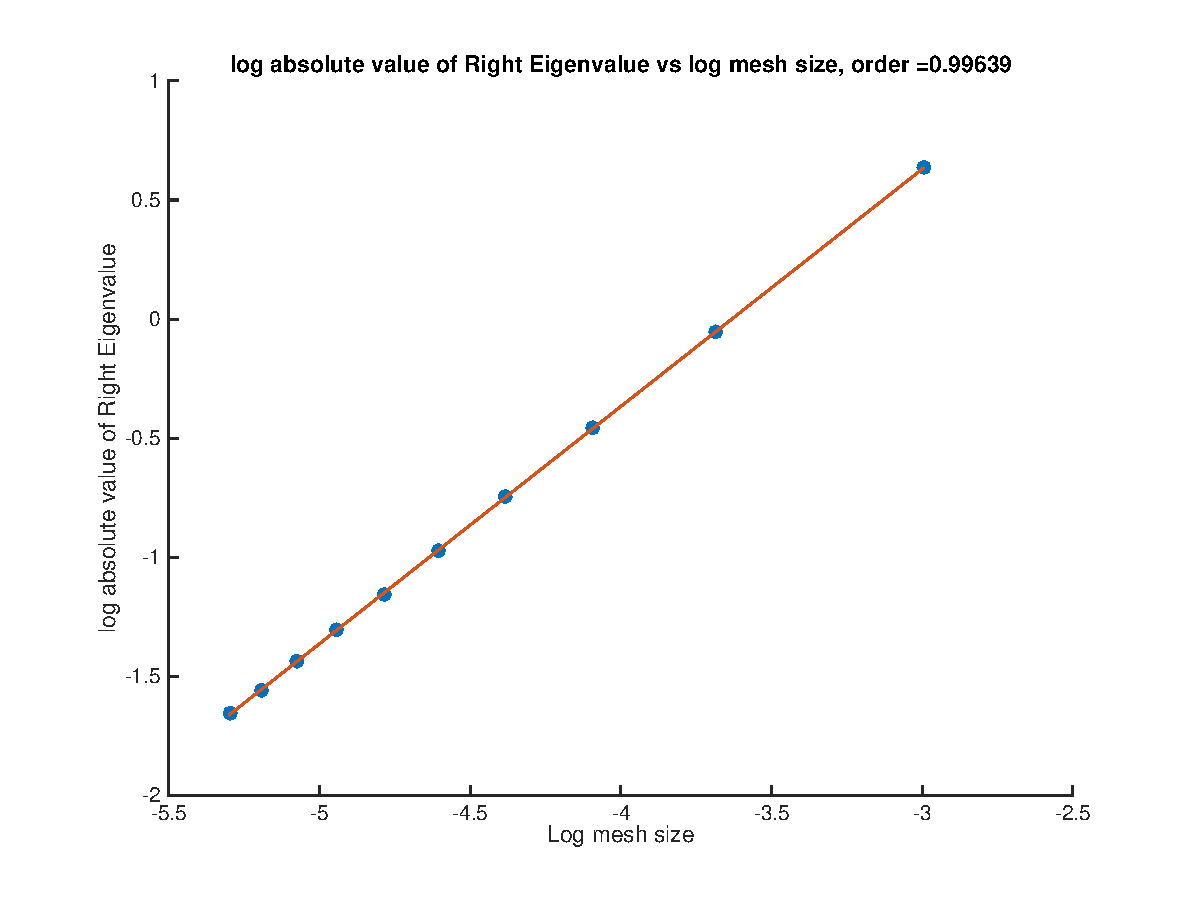
\includegraphics[width=8.5cm]{1double2fdrighteigabs}
\end{figure}

Next let's look at the Left Eigenvalue. It looks like the imaginary part is converging to something like 0.670. First, check to make sure the real part is converging to 0 like before.

\begin{figure}[H]
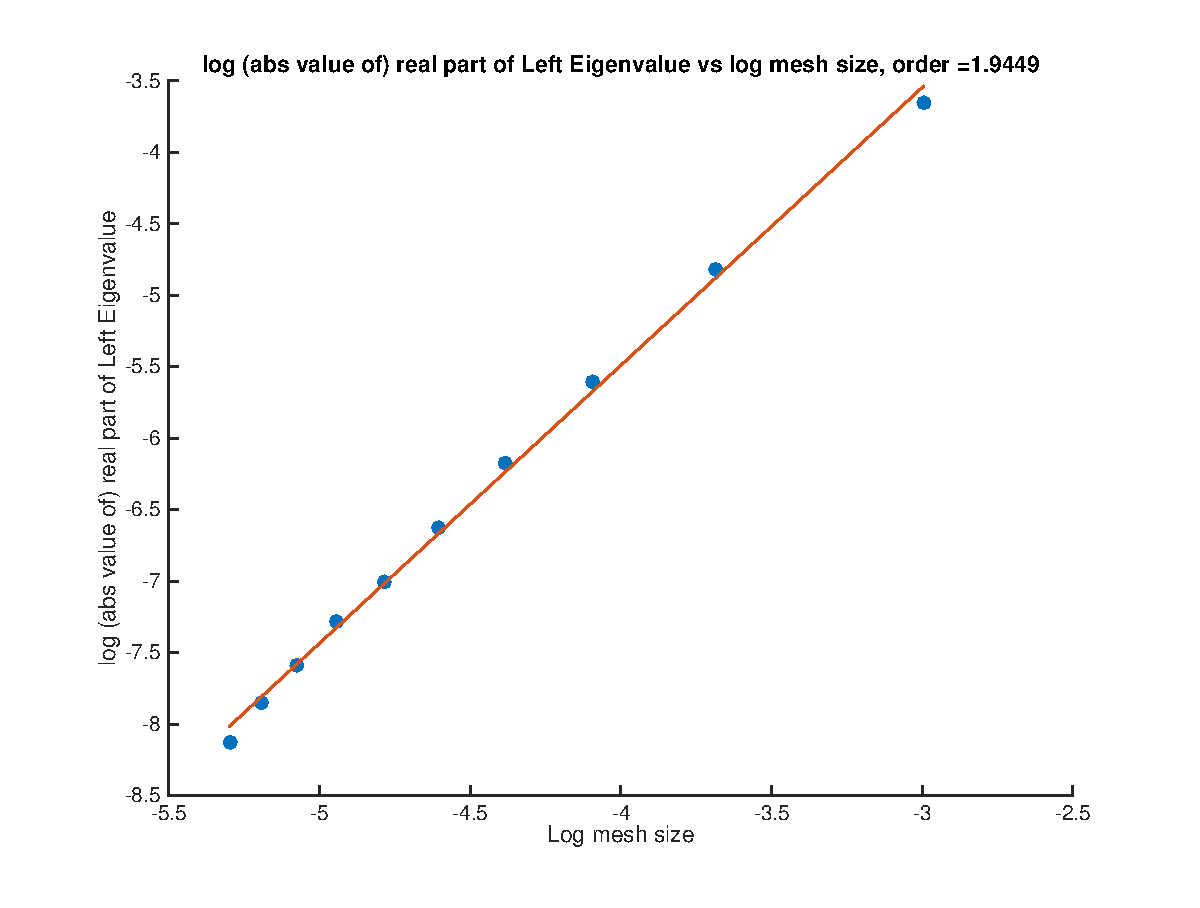
\includegraphics[width=8.5cm]{1double2fdlefteigreal}
\end{figure}

We get 2nd order convergence of the real part of the Left Eigenvalue to 0 (as before), so this is good. Before we deal with the imaginary part, let's look at Fourier.

\begin{figure}[H]
\begin{tabular}{l|ll}
$N$    & Left eigenvalue      &  Right eigenvalue    \\ \hline
  128  &     -0.4647e-05 + 0.6430i &       3.3100e-05  +  0.0403i \\ 
  256  &      0.1733e-05 + 0.6423i &      -1.2287e-11  +  2.2605e-05i \\ 
  512  &      0.1735e-05 + 0.6423i &      -3.0773e-04  +  0i\\ 
  1024 &      0.1692e-05 + 0.6423i &      -4.0926e-09  +  5.9097e-04i\\
  2048 &      2.7662e-06 + 0.6423i &      1.9930e-06   +  0.0062i
\end{tabular}
\end{figure}

We don't get a nice convergence pattern here, most likely since we are near max precision like we were for Double Pulse 1. For the Left Eigenvalue, the imaginary part seems to rapidly converge to 0.6423. The real part is always of order of magnitude $1e-05$, but this deviation from 0 is likely due to the numerical method since the finite difference method converges nicely and since this seems to be about the order of magnitude of this method from what we saw above.\\

What we can do is use \texttt{fsolve} on the eigenvalue problem $(J -\lambda f) = 0$ ($J$ is Jacobian of problem linearized about double pulse). We set the eigenvalue to $0.6423i$ (i.e. get rid of the tiny real part), and use the eigenfunction we got as a starting point. Here is table of the max of the absolute value of the eigenvalue problem $J -\lambda f$ before and after \texttt{fsolve} for different grid sizes.

\begin{figure}[H]
\begin{tabular}{l|ll}
  $N$   &  $\max J -\lambda f$ before \texttt{fsolve}  &  $\max J -\lambda f$ after \texttt{fsolve} \\ \hline
  256   &     4.1982e-11 &   1.4055e-07   \\ 
  512   &     1.5391e-09 &   3.2847e-07   \\ 
  1024  &     5.4523e-08 &   1.8613e-07   \\
  2048  &     2.5028e-06 &   6.0373e-07   \\
\end{tabular}
\end{figure}
We see that by the time we get to 2048 grid points, the \texttt{fsolve}d eigenvector is actually better than the initial one! Even more evidence that these eigenvalues are pure imaginary. Here is a plot of the real and imaginary parts of the corresponding eigenfunction (after \texttt{fsolve}, 2048 grid points); the eigenfunctions are in the exp weighted space.
\begin{figure}[H]
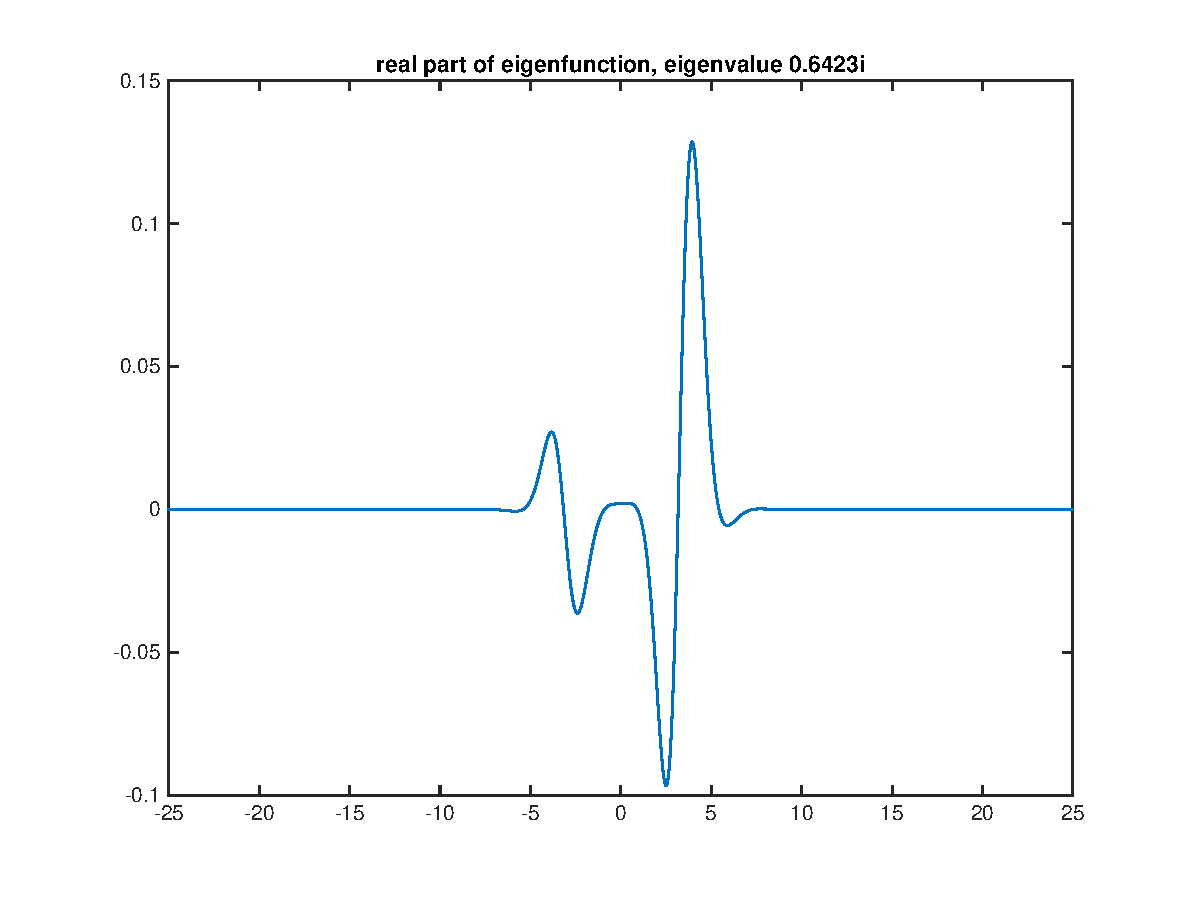
\includegraphics[width=8.5cm]{1double2eigenfnreal}
\includegraphics[width=8.5cm]{1double2eigenfnimag}
\end{figure}
We can convert the eigenfunction back to the unweighted space by multiplying it by $e^{-ax}$, where $a = 0.2$ here. Here are the real and imaginary parts of the unweighted eigenfunctions.
\begin{figure}[H]
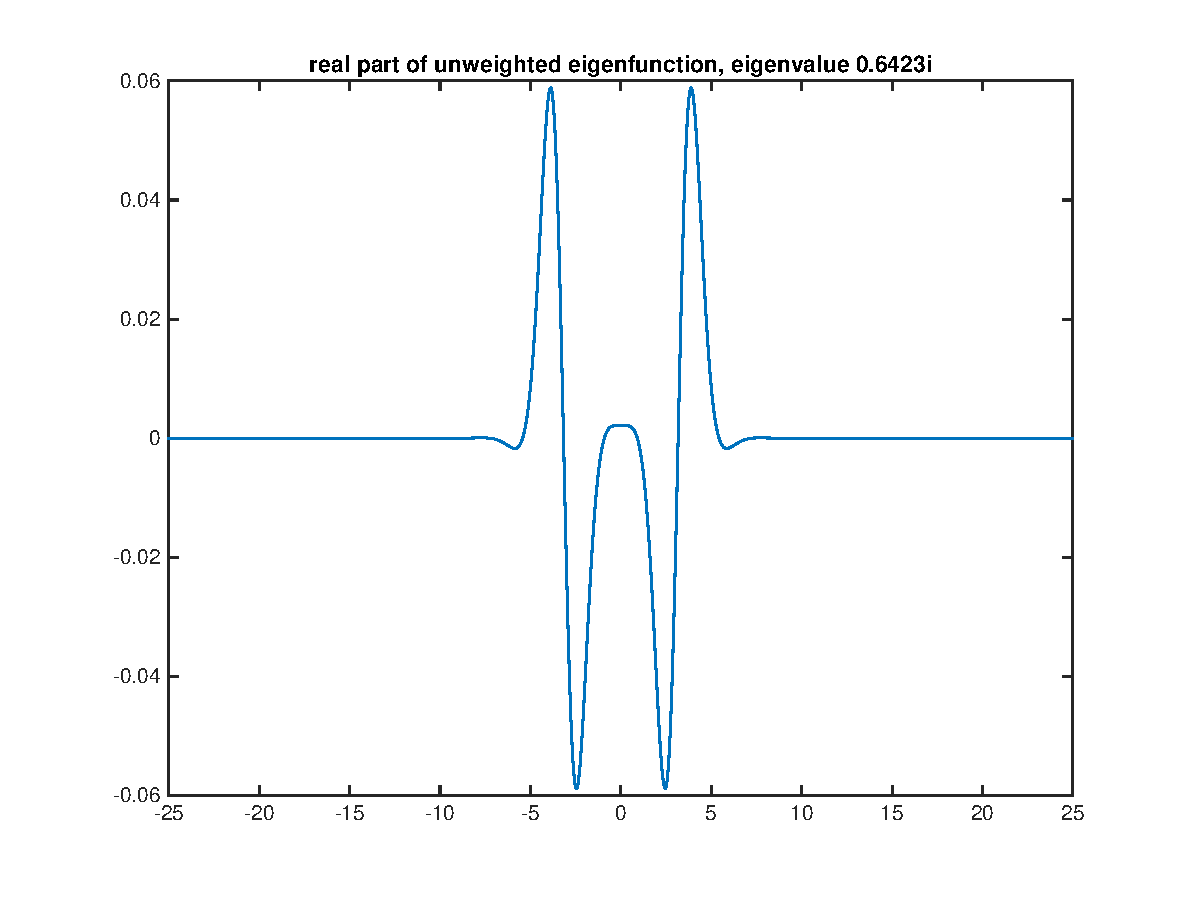
\includegraphics[width=8.5cm]{1double2eigenfnrealunweighted}
\includegraphics[width=8.5cm]{1double2eigenfnimagunweighted}
\end{figure}

Now that we know what we are looking for, we can try to fish out this eigenvalue from the essential spectrum in the unweighted space. (The essential spectrum in the nondiscretized world is the entire imaginary axis, which makes this difficult.) As above, we can use \texttt{fsolve} to get rid of the tiny real part of the eigenvalue and give us a pure imaginary eigenvalue. Here is a table of the results.

\begin{figure}[H]
\begin{tabular}{l|lll}
  $N$   & eigenvalue &  $\max J -\lambda f$ before \texttt{fsolve}  &  $\max J -\lambda f$ after \texttt{fsolve} \\ \hline
  256   &  1.6239e-11 + 0.6423i  & 7.6305e-11   &    1.1220e-11  \\ 
  512   & -3.2265e-10 + 0.6423i  &  2.0980e-09  &   3.0428e-10  \\ 
  1024  &  8.7075e-09 + 0.6423i  &  4.4871e-08  &  1.7600e-08 \\
\end{tabular}
\end{figure}
Now let's look at the corresponding eigenfunction and compare to what we got but ``unweighting'' the weighted eigenfunction. They are very similar, which is good.
\begin{figure}[H]
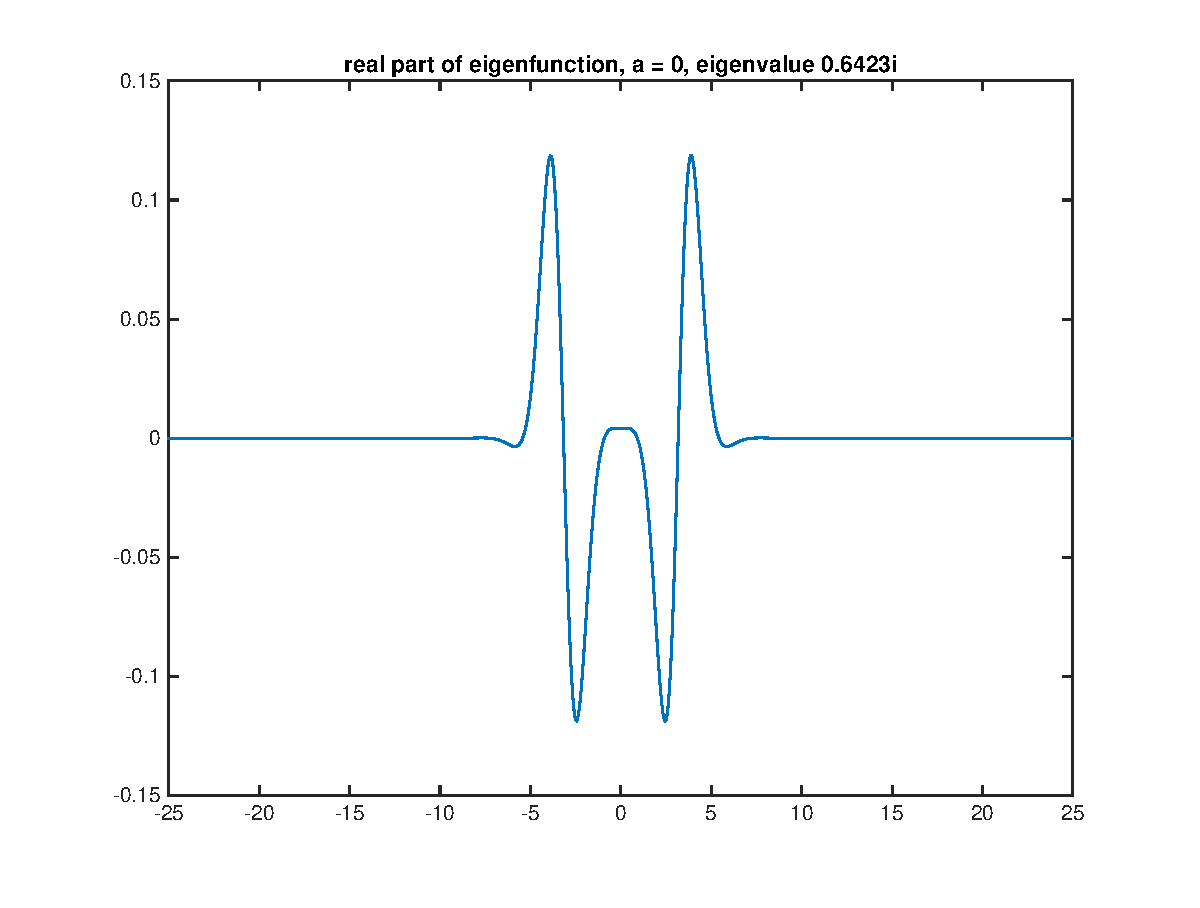
\includegraphics[width=8.5cm]{1double2a0eigenfnreal}
\includegraphics[width=8.5cm]{1double2a0eigenfnimag}
\end{figure}
It it interesting to note what eigenvalues we have on the imaginary axis between $-0.6423i$ and $0.6423i$. There are two eigenvalues at 0 (to numerical precision) whose eigenfunctions are the derivative of the double pulse. There are also two eigenvalues at 0 whose eigenfunctions are essentially nonlocalized garbage.\\

We can also look at the integrals of these eigenfunctions. We use the eigenfunctions found in the unweighted space (after \texttt{fsolve}) and integrate using trapezoid rule (\texttt{trapz}). 
\begin{figure}[H]
\begin{tabular}{l|lll}
  $N$   & eigenvalue &  Integral of Eigenfunction & Abs Value of Integral \\ \hline
  256   & 0.6423i  &  6.9713e-07 + 1.0313e-08i & 6.9721e-07 \\ 
  512   & 0.6423i  &  2.4639e-07 + 7.3560e-09i & 2.4650e-07 \\ 
  768   & 0.6423i  &  1.3369e-07 + 7.0911e-09i & 1.3388e-07 \\
  1024  & 0.6423i  &  9.0563e-08 + 1.4987e-08i & 9.1795e-08 \\
\end{tabular}
\end{figure}

Looking the table, the integral of the imaginary part does not have a nice convergence trend to 0. However if we plot the log absolute value of the integral versus the log of the mesh size, we get a nice straight line, so this is good.

\begin{figure}[H]
\includegraphics[width=8.5cm]{1double2fouriereigenfnabsintegralN}
\end{figure}

The order of convergence is roughly 1.5, which is about the same as for the eigenfunction of Double Pulse 1, but I have no idea what this means. We can also vary the domain length $L$, keeping the mesh size constant.

\begin{figure}[H]
\begin{tabular}{l|llll}  
  $N$  & $L$    &  Eigenvalue &  Integral of Eigenfunction  & Abs Value of Integral   \\ \hline
  256  &  25    &   0.6423i   &  6.9713e-07 + 1.0313e-08i & 6.9721e-07 \\ 
  512  &  50    &   0.6423i   &  3.6105e-07 + 5.5240e-09i & 3.6109e-07 \\ 
  768  &  75    &   0.6243i   & -2.7143e-07 - 4.2293e-09i & 2.7146e-07 \\
  1024 &  100   &   0.6423i   &  2.4759e-07 + 3.8597e-09i & 2.4762e-07 \\
\end{tabular}
\end{figure}
The real part and the absolute value of the integral are both getting smaller, although we don't have a nice relation like we for the mesh size. \\

We can also keep the grid size fixed at $N = 2048$ and vary the domain length $L$. Unfortunately, unlike the case for Double Pulse 1, there is not any nice relationship here.

\begin{figure}[H]
\begin{tabular}{l|lll}
  $N$   &  $L$ & Integral of Eigenfunction & Abs Value of Integral \\ \hline
        &   $1.0e-06 *$         & $1.0e-06 *$ \\
  2048  & 25    &   0.0368 - 0.2159i &   0.2190 \\ 
  2048  & 50    &  -0.0450 + 0.0122i &   0.0467 \\ 
  2048  & 75    &   0.0624 - 0.0010i &   0.0624 \\
  2048  & 100   &   0.0875 + 0.0023i &   0.0876 \\
\end{tabular}
\end{figure}


\subsubsection*{Double Pulse 3}
Here we use Fourier spectral methods with 1024 grid points. We already know we have a pair of real eigenvalues ($\lambda = \pm 0.1176$), but we want to see the eigenfunctions.

\begin{figure}[H]
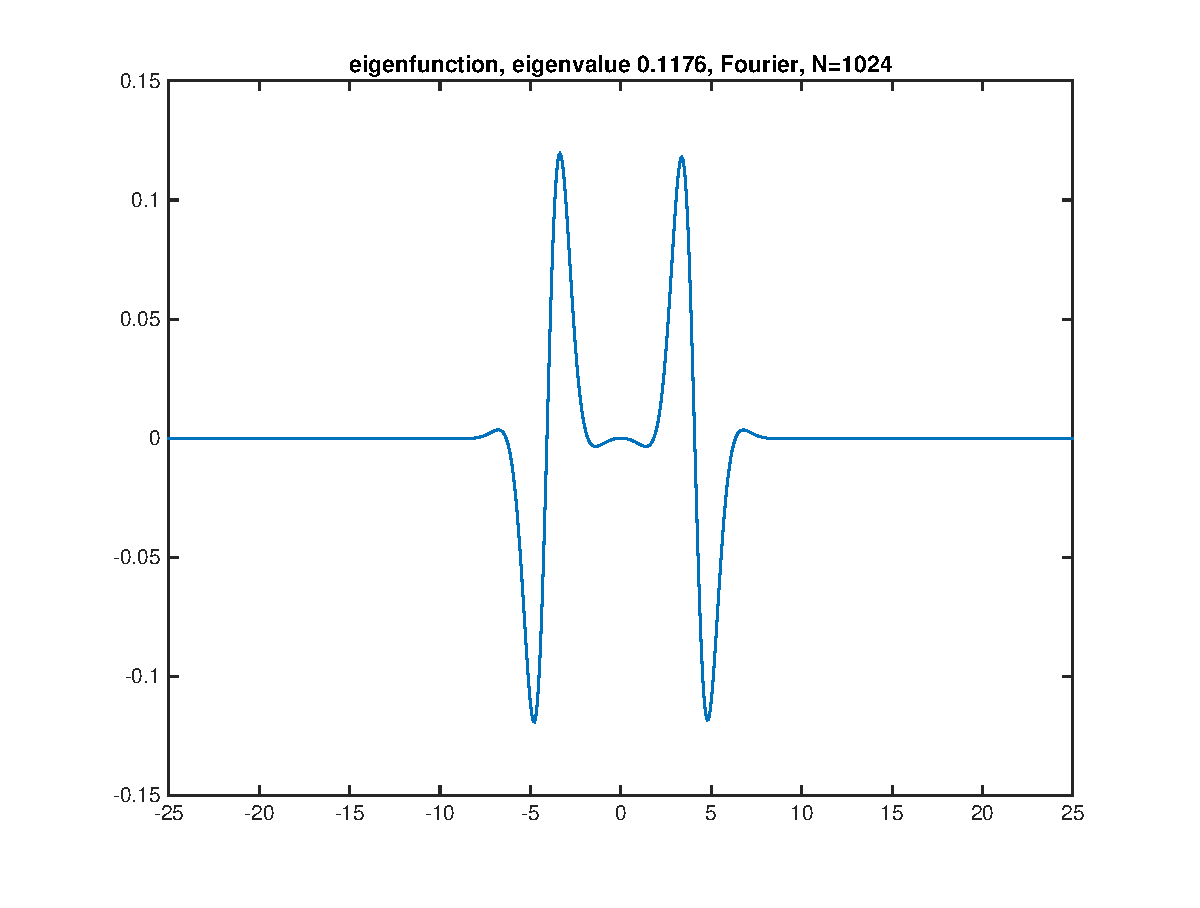
\includegraphics[width=8.5cm]{1double3fouriereigenfnplus}
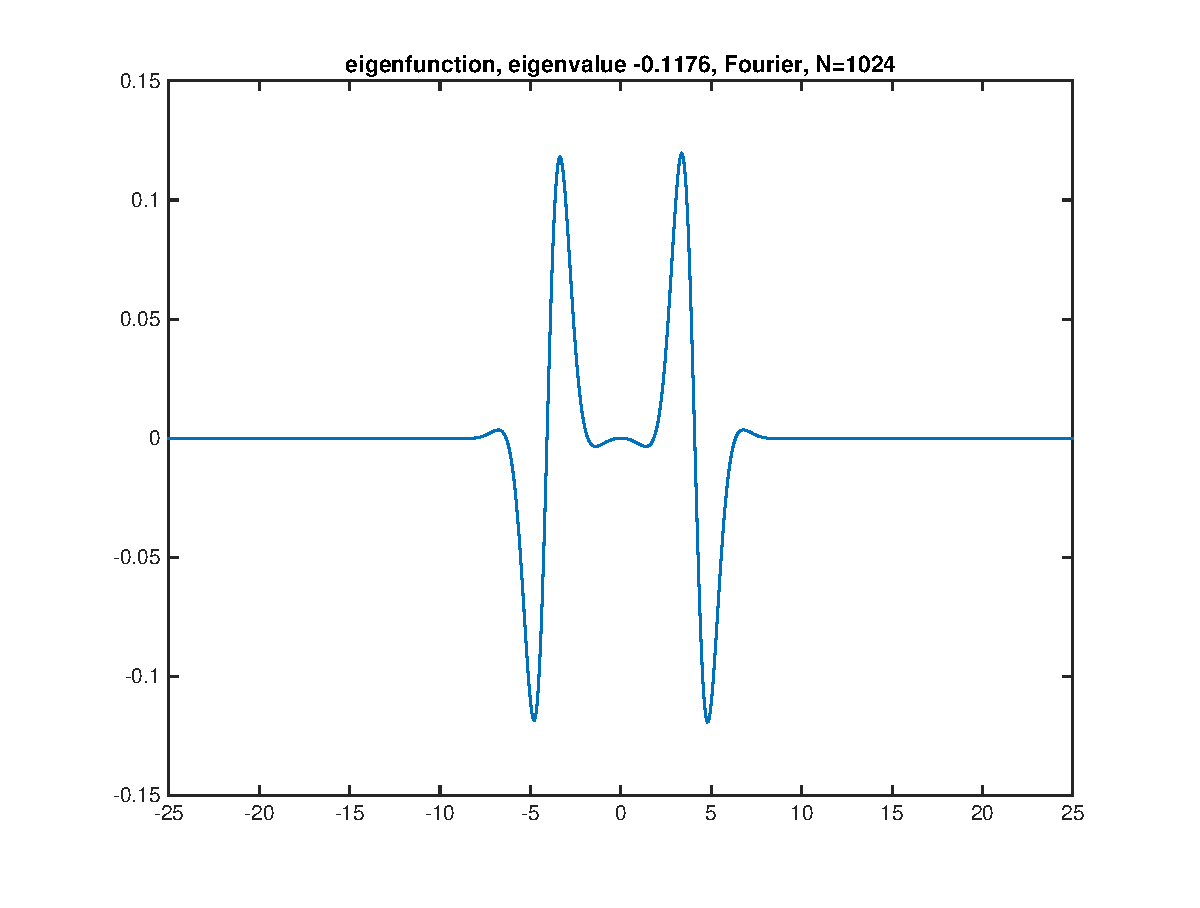
\includegraphics[width=8.5cm]{1double3fouriereigenfnminus}
\end{figure}
The two eigenfunctions are again reflections of each other about the y-axis. They are very close to symmetric about the y-axis, but not quite. The two peaks are not the same height; for the positive eigenvalue, the left peak is higher both for Double Pulse 3 and Double Pulse 1. I'm not sure what this means, but it is consistent, so that is good.

\subsubsection*{Double Pulse 4}
Finite difference methods do not do well here (probably because the eigenvalues are too small), so we will use Fourier. Given what we learned from Double Pulse 2, this should be fine. Another advantage of Fourier is that the differentiation matrices are always small enough to use \texttt{eig} instead of \texttt{eigs}. We will focus only on the Left Eigenvalue, since that's the one we are interested in. Here is a table of the Left Eigenvalue, together with the max error of the eigenvalue problem before and after \texttt{fsolve}.

\begin{figure}[H]
\begin{tabular}{l|lll}
  $N$   & left eigenvalue &  $\max J -\lambda f$ before \texttt{fsolve}  &  $\max J -\lambda f$ after \texttt{fsolve} \\ \hline
  256   &  -1.5832e-11 + 0.0215i &  6.7141e-11  &  1.3100e-11   \\ 
  512   &   7.1199e-10 + 0.0215i &  1.3103e-09  &  7.2288e-10   \\ 
  1024  &  -1.4488e-08 + 0.0215i &  4.7470e-08  &  2.2036e-08 \\
\end{tabular}
\end{figure}

Again, for the pre-\texttt{fsolve} version, the real parts are very close to 0, and the max error decreases (for all numbers of grid points we tried) after we use \texttt{fsolve} to make the real part of the eigenvalue 0. The real and imaginary parts of the eigenfunction (after \texttt{fsolve}) are plotted below.

\begin{figure}[H]
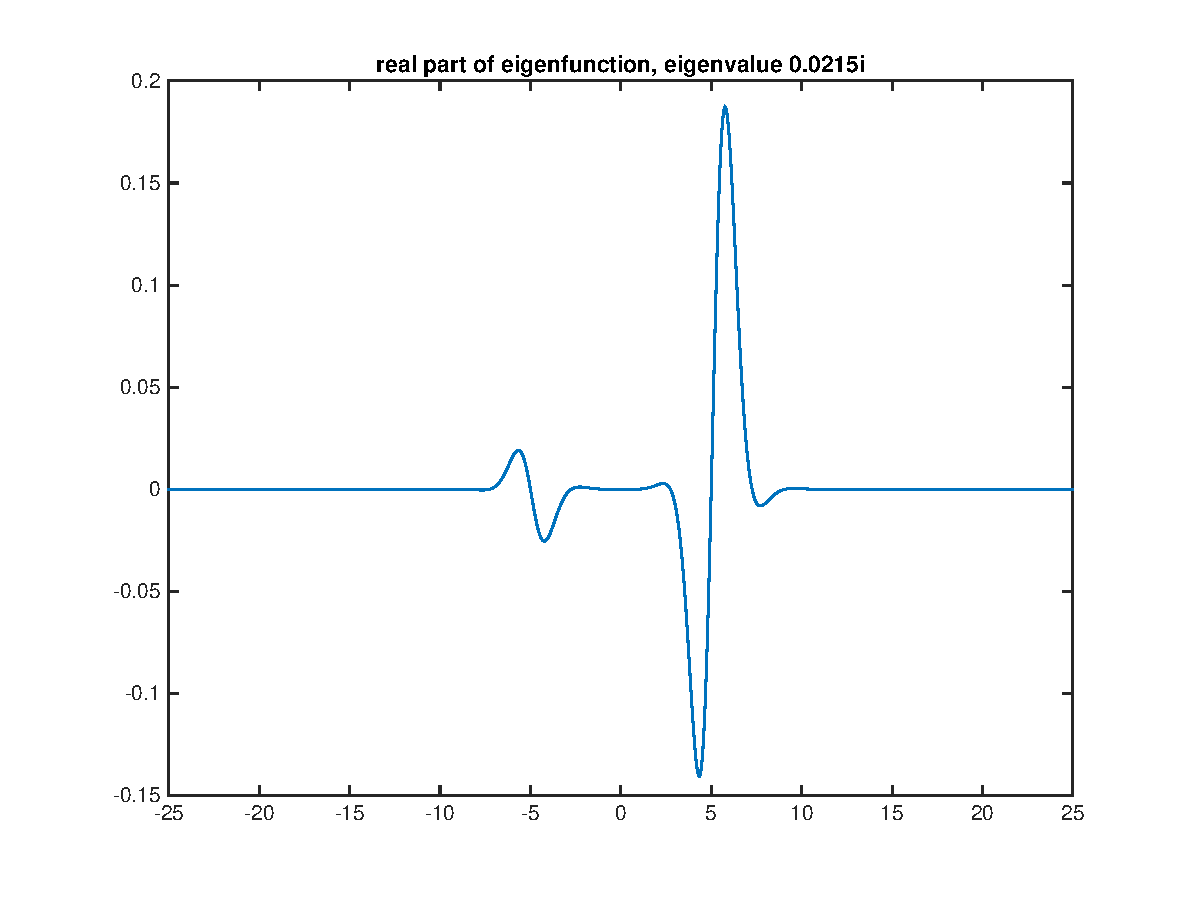
\includegraphics[width=8.5cm]{1double4eigenfnreal}
\includegraphics[width=8.5cm]{1double4eigenfnimag}
\end{figure}
Doing exactly what we did above, here are the real and imaginary parts of the unweighted eigenfunctions.
\begin{figure}[H]
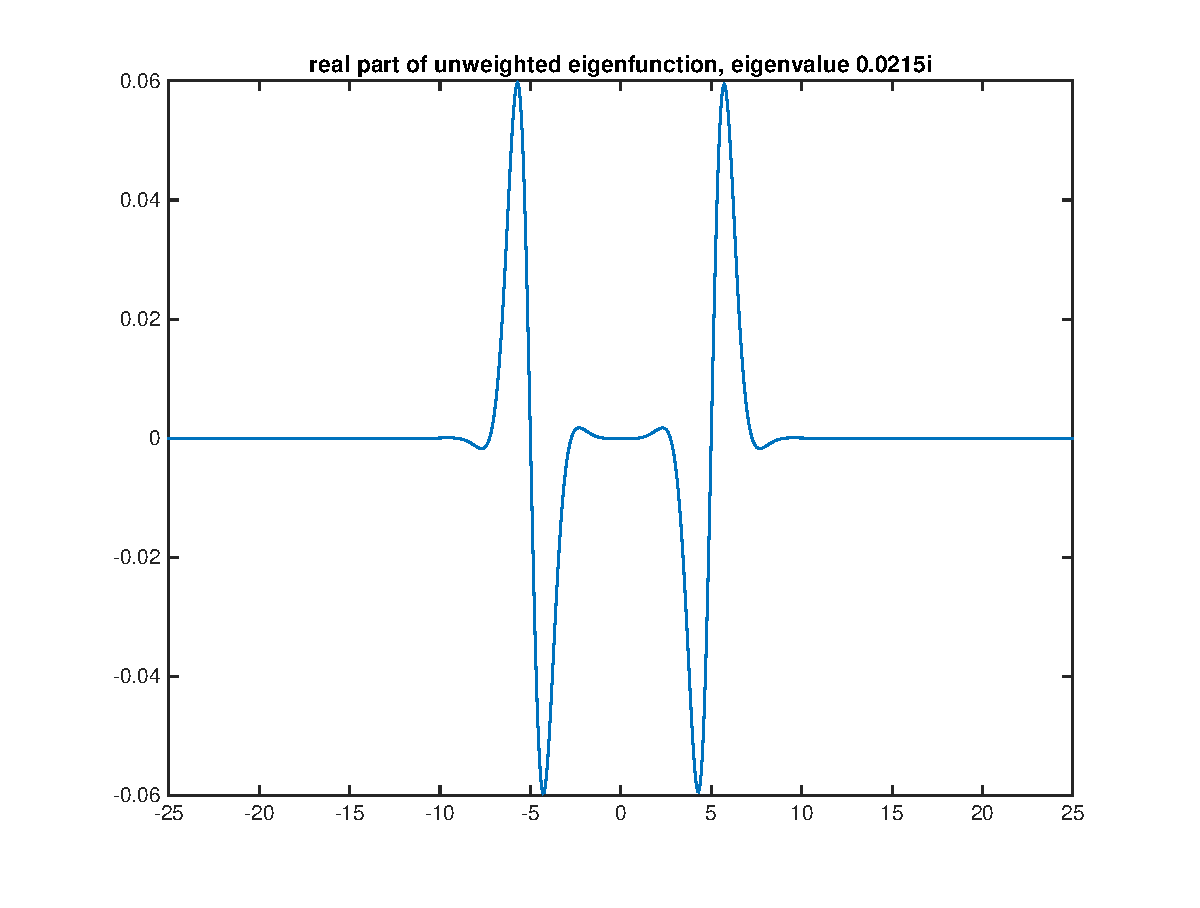
\includegraphics[width=8.5cm]{1double4eigenfnrealunweighted}
\includegraphics[width=8.5cm]{1double4eigenfnimagunweighted}
\end{figure}

We can do the same thing we did for Double Pulse 2, and fish out these eigenvalues from the absolute spectrum in the unweighted space. If we do that, we find two eigenvalues on the imaginary axis at $\pm 0.0215$, just as we expected. (They have real parts of order of magnitude $1e-9$ which can be eliminated with \texttt{fsolve}). If we plot the corresponding eigenfunctions, we get:
\begin{figure}[H]
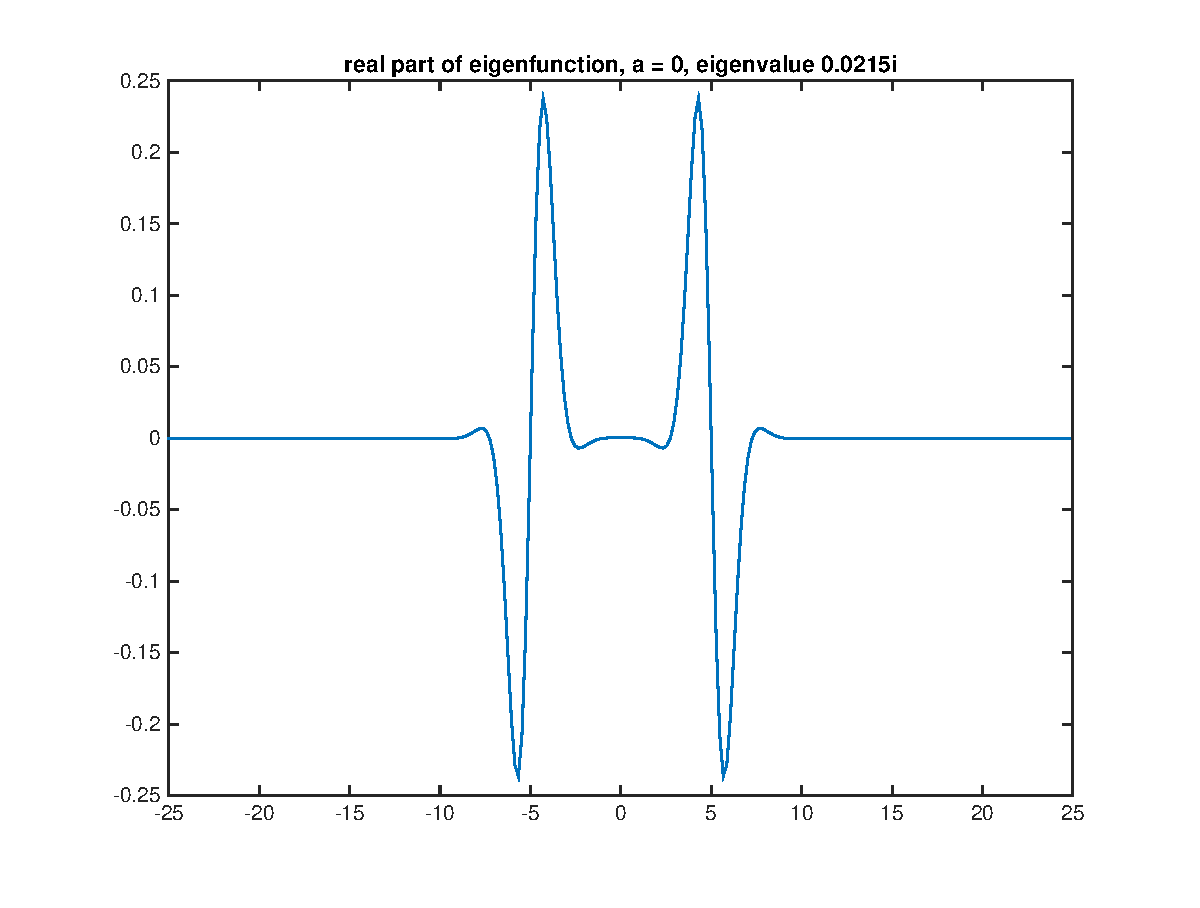
\includegraphics[width=8.5cm]{1double4a0eigenfnreal}
\includegraphics[width=8.5cm]{1double4a0eigenfnimag}
\end{figure}
This is the negative of the version we found when we ``unweighted'' the weighted eigenfunction, but that's ok since eigenfunctions are only defined up to a constant multiple. Also multiplying by -1 doesn't change the norm, and these are all normalized.


\section*{10 March 2017}
\subsection*{Shallow water equation}
This is the following 5th order PDE:
\[
u_t + \partial _x\left( \frac{2}{15}u_{xxxx} - b u_{xx} + \frac{3}{2}u^2 + \frac{1}{2}u_x^2 + u u_{xx} \right) = 0
\]
As usual, we take a traveling wave solution $u = u(x + ct)$. We showed before that we can construct double pulses with eigenvalue patterns identical to that of the 5th order KdV equation. Now we repeat what we did above with this equation. We take $b = 2.5$ since Sanstede (2015) suggests that to have multipulses we need to choose $b > 2$. For this value of $b$, we have a known solution for $c = c_*(b) = 1.8$. Somewhere above $c = 10$, the eigenvalues of the eigenvalues of the linearization about the zero-solution become complex, so we run continuation code in the parameter $c$ until we reach $c = 20.4414$. \\

We then construct double pulses. For this equation, finite difference are not accurate enough, and in fact we cannot get \texttt{fsolve} to converge for $N > 5000$ or so. Thus we will use Fourier spectral methods. Given what we observed above, this is a good choice. Continuation code is run with $N = 512$ grid points and domain length $L = 15$. It looks like we need at least $N = 512$ grid points with Fourier to get good results.

\subsubsection*{Double Pulse 1}
As expected, we get two real eigenvalues which are negatives of each other.
\begin{figure}[H]
\begin{tabular}{l|ll}
$N$    & Positive real eigenvalue      &  Difference      \\ \hline
  512  &        11.3090  &                  \\ 
  1024 &        11.3090  &      8.2311e-07  \\
\end{tabular}
\end{figure}
These values are close, so we did not go to higher numbers of grid points. The corresponding eigenfunctions are reflections of each other about the y-axis, as expected. They are also qualitatively similar to the eigenfunctions for Double Pulse 1 of the KdV equation.

\begin{figure}[H]
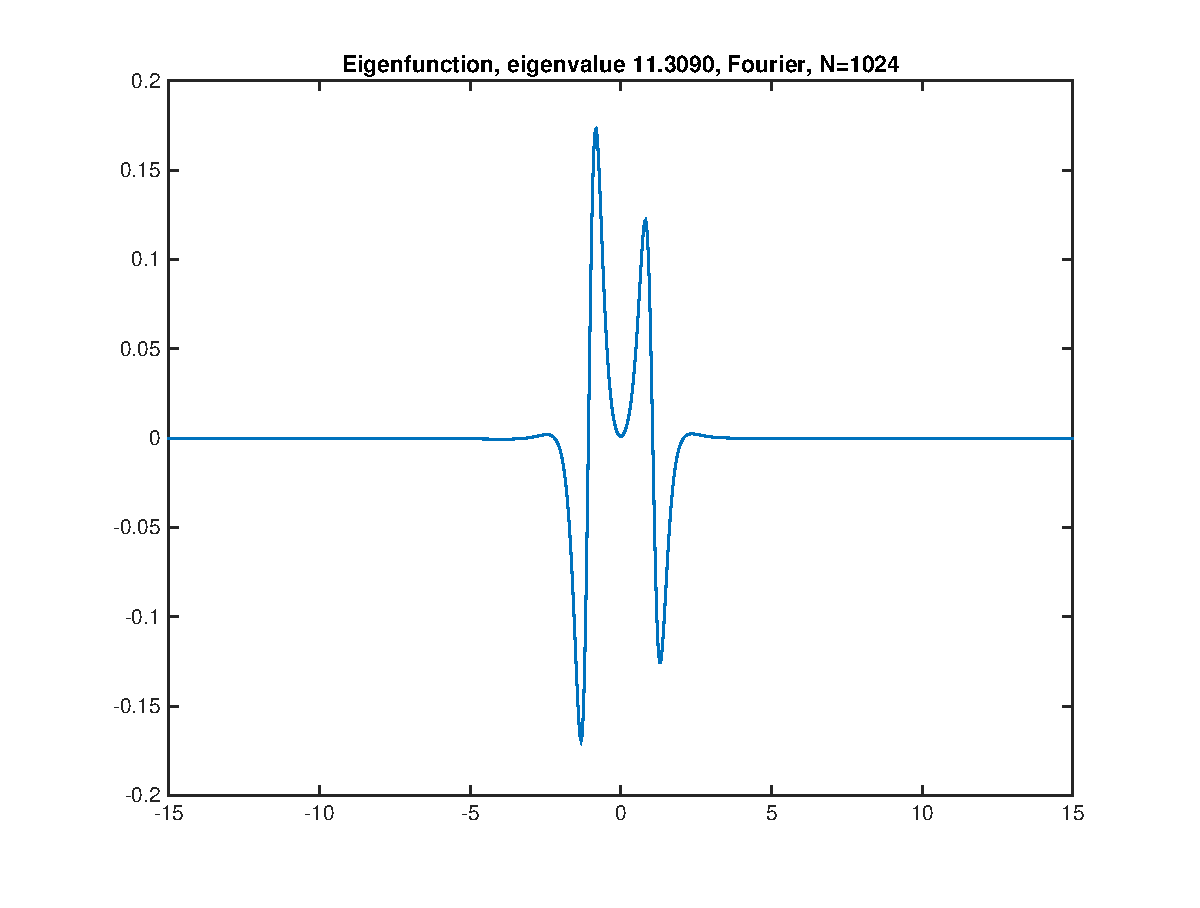
\includegraphics[width=8.5cm]{Sh1double1eigenfnplus}
\includegraphics[width=8.5cm]{Sh1double1eigenfnminus}
\end{figure}

\subsubsection*{Double Pulse 2}
As expected, if we take an exponentially weighted space ($a = 0.2$, same as for KdV, provides good separation from the absolute spectrum), we get a pair of complex conjugate eigenvalues which are approximatley on the imaginary axis, and a pair of eigenvalues near 0. The pair near 0 have eigenfunctions which look like the derivative of the double pulse, as expected, so we will ignore them for now and focus on the other pair. We only take the eigenvalue with positive imaginary part, since the two make a complex conjugate pair. As with the KdV equation, we can successfully run the eigenfunction through \texttt{fsolve} to get rid of the real part of the eigenvalue. For the \texttt{fsolve}, we are now requiring the norm of the eigenfunction to be 1 (\texttt{eig} and \texttt{eigs} output normalized eigenfunctions, so this makes sure we don't accidentally converge to the 0 function; not sure how much diffence it really makes, but certainly does not hurt).

\begin{figure}[H]
\begin{tabular}{l|lll}
  $N$   & Eigenvalue &  $\max J -\lambda f$ before \texttt{fsolve}  &  $\max J -\lambda f$ after \texttt{fsolve} \\ \hline
  512   &   4.6663e-07 +  0.1533i &   2.6353e-09  &  5.6233e-10   \\ 
  768   &   4.4082e-07 +  0.1534i &   7.1376e-08  &  4.9443e-09   \\
\end{tabular}
\end{figure}

For more grid points, it was taking \texttt{fsolve} a while to converge. Since the results look good, didn't feel the need to go to more grid points at this time.\\

The real and imaginary parts of the eigenfunction (after \texttt{fsolve}) are plotted below.
\begin{figure}[H]
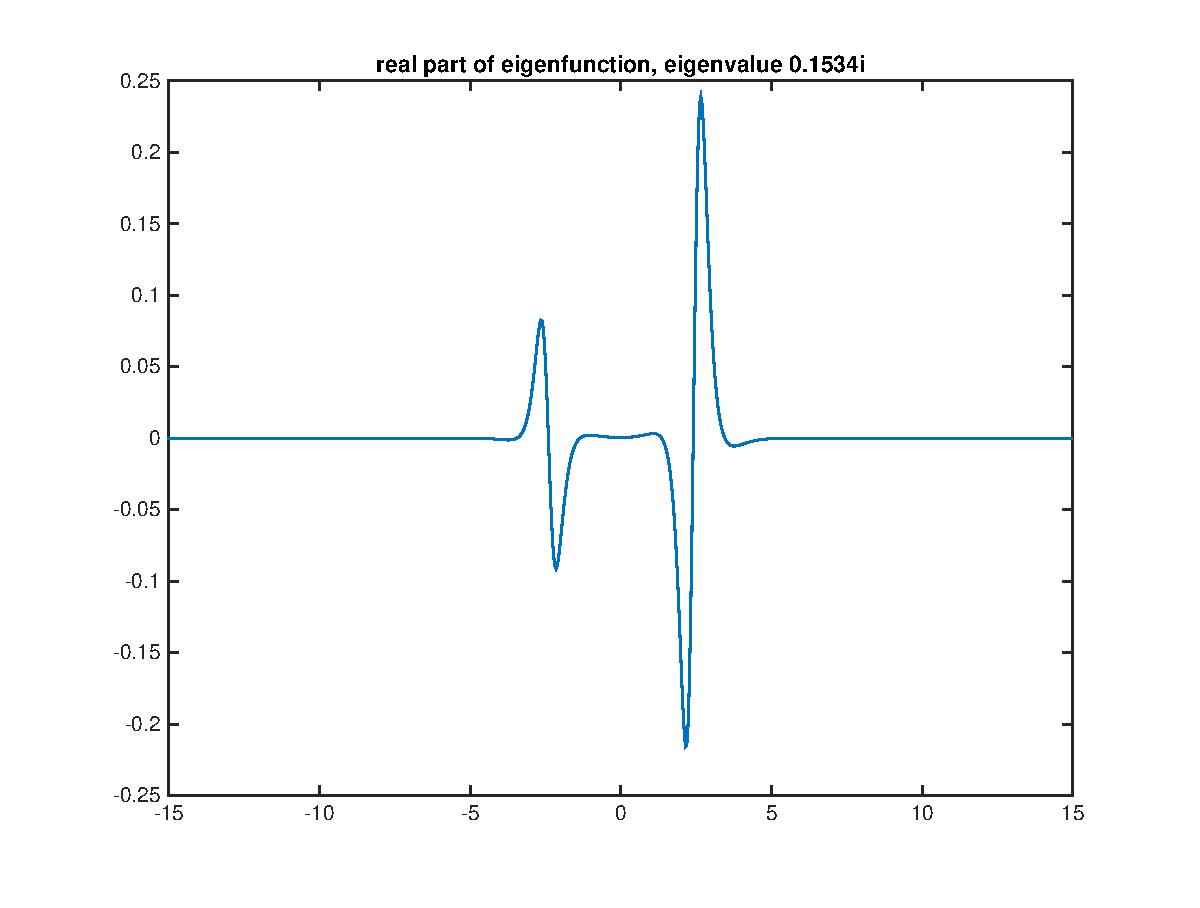
\includegraphics[width=8.5cm]{Sh1double2eigenfnreal}
\includegraphics[width=8.5cm]{Sh1double2eigenfnimag}
\end{figure}
Doing exactly what we did above, here are the real and imaginary parts of the unweighted eigenfunctions.
\begin{figure}[H]
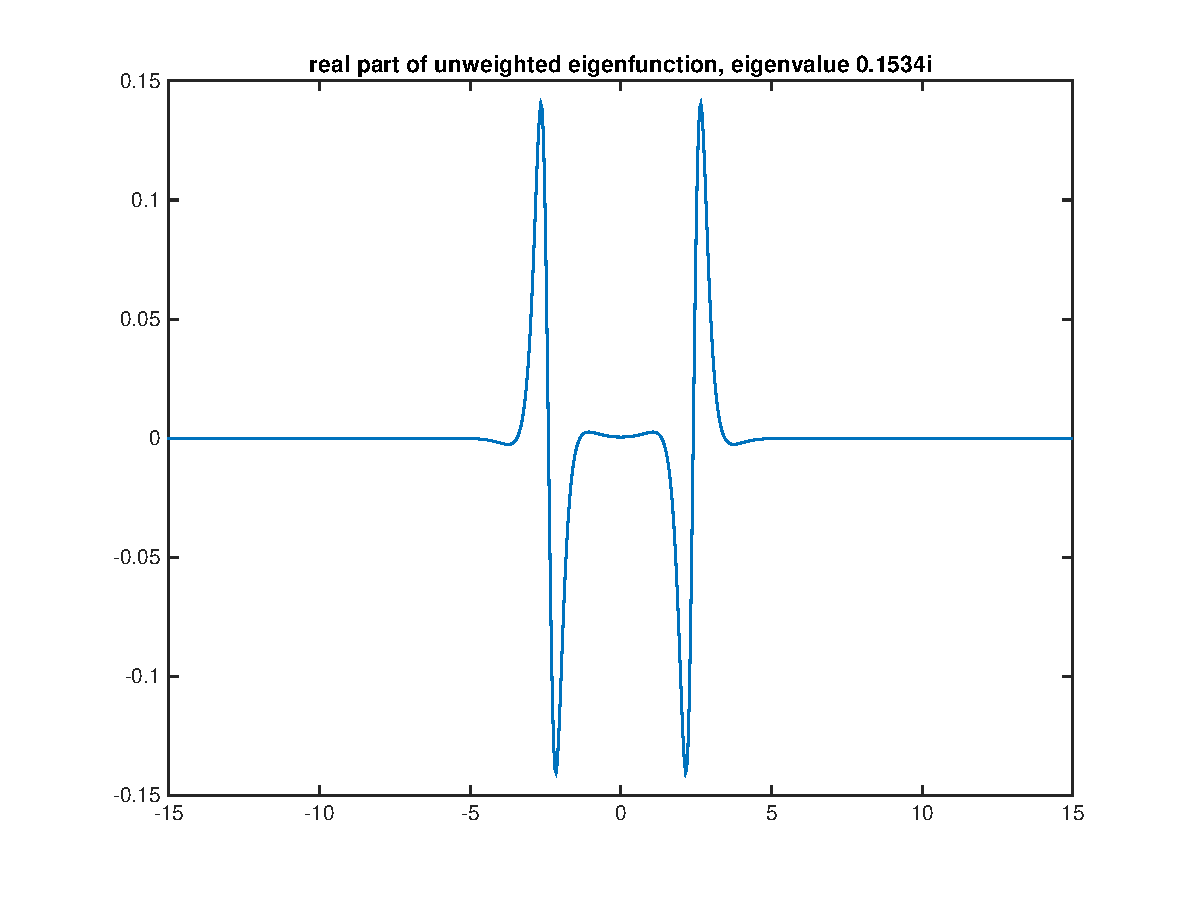
\includegraphics[width=8.5cm]{Sh1double2eigenfnrealunweighted}
\includegraphics[width=8.5cm]{Sh1double2eigenfnimagunweighted}
\end{figure}

\section*{14 March 2017}
\subsection*{Chardard}
I took a look at the Chardard papers to see where they reference double pulse Eigenvalues for KdV5. If we look at Chardard, 2009 (Computational aspects of the Maslov index of solitary waves), this topic is discussed in Section 15.1 (p. 39):
\begin{quote}
The Maslov index does not give any information about the purely imaginary eigenvalues, and so to determine their number, a calculation of the spectral problem is necessary. Some results on this are reported by Chardard [15]. There it is found that when l is odd, there are eigenvalues with non-zero imaginary part, but they appear to have very small real parts. Further results are necessary to be certain about the spectral stability of 2 pulse solitary waves when l is odd.
\end{quote}
The reference is to Chardard's doctoral thesis \textit{Stabilite des ondes solitaires} (2009). This is freely available on his website and is (fortunately) in English. Chapter 3 deals with the Kawahara equation, which is a generalization of the 5th order KdV. The steady-state form, for traveling waves of speed $c$, after integrating once, is:
\[
u_{xxxx} - Pu_{xx} + cu - u^{q+1} = 0
\]
Our 5th order equation is the special case of $P =1, q = 1$. Multipulse solutions should exist for $P \geq -2$, so we are good. Our double pulses look qualitatively like those in Figure 3.7 (p. 68), although this figure is for $P = -1.5$. Note that our Double Pulse 0 is labeled pulse 1 in that figure.\\

In section 3.6 (p. 76), Chardard finds the eigenvalues of the linearized 5th order operator by numerically computing and finding zeros of the Evans function. Two-pulse solutions with an odd index (I believe this is the Maslov index, but this corresponds to our odd-numbered double pulses above) should have an unstable real eigenvalues; Chardard found that with his numerics, and we found that too. For two-pulse solutions with even index, however, Chardard (2009) says (p.77):
\begin{quote}
However, we find for most cases that there is a pair of complex eigenvalues with a small real
part associated to each even index. Dividing by two the step and multiplying by two the length
of the interval did not shift significantly the eigenvalue.
\end{quote}
So, basically Chardard's numerics give a different result from our numerics. His small real parts don't go away, whereas we can get ours to go away either using \texttt{fsolve} or by a convergence argument. At this point, I'm not sure who is correct, since if there were a real part to these eigenvalues, it would be tiny.

\end{document}

